\noindent
{\bf High-Fidelity Simulations on DOE Leadership Computers.}
  DOE's current- and next-generation leadership computers employ nodes that
  feature high-performance GPUs.  
We have recently demonstrated that it is possible to simulate a single
flow-through time for the thermal-hydraulics of a full pebble-bed reactor core
(352,000 pebbles) in just six hours of wall-clock time on using 27648 
NVIDIA V100s on ORNL's Summit \cite{sc22}.  This is an significant acheivement
as it involves updating a quarter-trillion degrees-of-freedom at $\approx$ 0.3
seconds per step.  The software that enables this achievement is {\em NekRS},
which is the GPU-oriented version of the highly-scalable thermal-fluids code,
Nek5000.  NekRS is being developed under DOE's Center for Efficient Exascale
Discretizations (CEED) and sustains $\approx$ 0.5--1.0 TFLOPS ($10^{12}$
floating point operations per second) per MPI rank on current pre-exascale
platforms and 80\% parallel efficiency at about 2M grid points per rank.
Consequently, a 51B grid-point problem such as the pebble-bed reactor of Fig.
\ref{fig:pbr} can effectively use $P$=25,000 GPUs. While such a calculation
fills all of Summit, it will require only a fraction of DOE's exascale
platforms, where we can anticipate running much larger problems, or running at
multiple points in the reactor design space.

Like Nek5000, NekRS is based on high-order body-fitted spectral element
discretizations that has minimal numerical dispersion and dissipation, which
are essential features for efficient simulation of turbulence.  Time-stepping
uses either a $k$th-order semi-implicit method ($k$=2 or 3) or a $k$th-order
characteristics scheme that allows Courant numbers significantly larger than
unity.  Fast Poisson solvers are critical to rapid simulation of reactor flows.
NekRS has an extensive suite of preconditioners for the pressure-Poisson
problem that are tailored to accelerator-based HPC platforms.  As part of the
Nek5000 source, NekRS supports all of the features of Nek5000, which include a
large variety of boundary conditions and an extensive tool set for data
analysis of turbulent heat transfer.



\begin{figure}[t!] \centering
    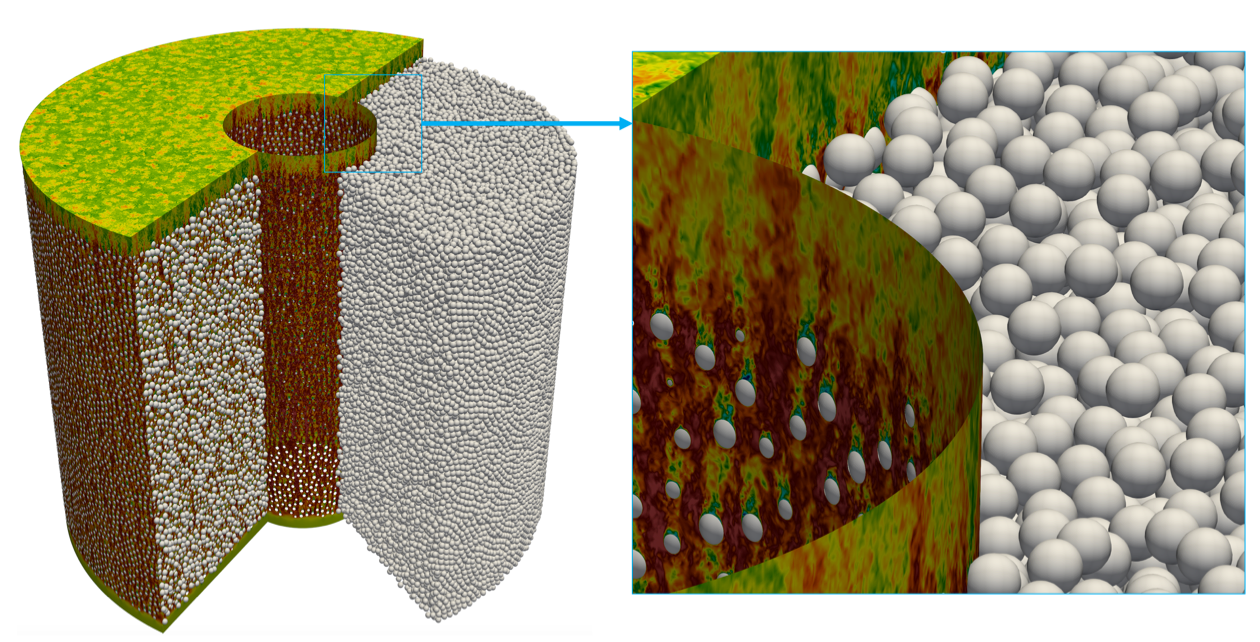
\includegraphics[width = 0.60\textwidth]{figs/pbr_pair.png}
    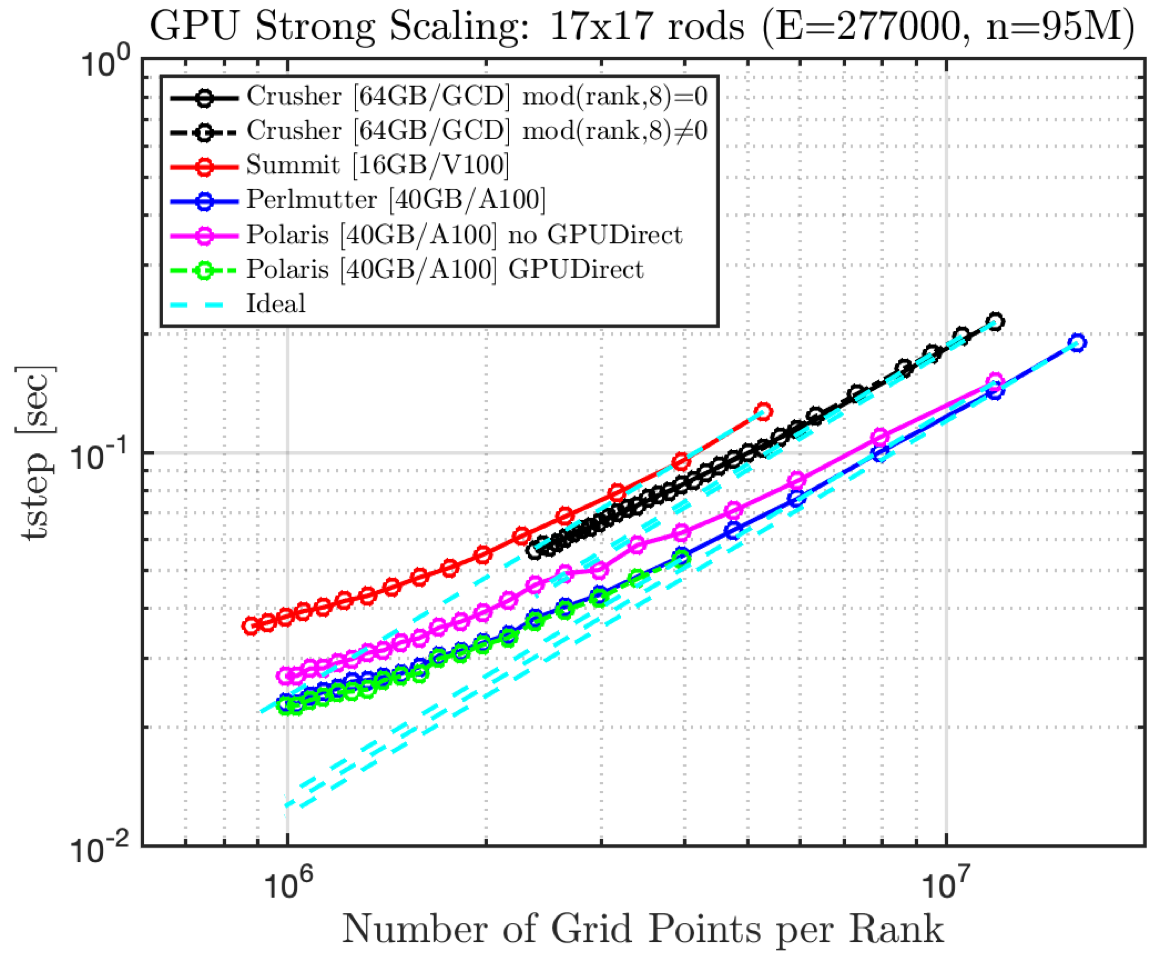
\includegraphics[width = 0.35\textwidth]{figs/nekrs_17x17_crusher_strong.png}
    \caption{(left) NekRS turbulent flow simulation results for a full reactor
core with 352625 pebbles.  The simulation comprised 51 billion gridpoints
($E$=99M spectral elements of order $p$=8).  On all of Summit (27648 NVIDIA
V100 GPUs), this simulation requires 0.36 seconds per step and would complete a
single flow-through time in just six hours \cite{sc22}. (Computation by
Yu-Hsiang Lan, ANL/UIUC.)
(right) NekRS strong-scaling on current-generation accelerator-based platforms:
AMD-MI250X-based Crusher (OLCF),
NVIDIA-V100-based Summit (OLCF),
NVIDIA-A100-based Perlmutter (NERSC),
NVIDIA-A100-based Polaris (ALCF).
The test problem is a 17$\times$17 rod-bundle with 95 million grid points.
(Simulations by Misun Min, ANL, and Yu-Hsiang Lan, ANL/UIUC.)
\label{fig:pbr}}
\end{figure}

